\begin{Answer}{1}
			$a)$ Các con vật có $4$ chân là Chó và Lợn.
			
			Do đó: Chó $\in A$; Gà $\notin A$; Lợn$ \in A$; Chim bồ câu $\notin A$; Rắn $\notin A$.
			
			$b)$ 3 phần tử thuộc tập hợp $A$ là: Trâu; Bò; Ngựa.
	
\end{Answer}
\begin{Answer}{3}
		$\bullet$	Cách 1: $M = \{0; 1; 2; 3; 4\}$.
		
		$\bullet$	Cách 2: $M = \{ y \mid y \in \mathbb{N},\, m y + 1 < 6\}$.
	
\end{Answer}
\begin{Answer}{4}
		\,\\
			\renewcommand{\arraystretch}{1.1}
			\begin{tabularx}{\textwidth}{|p{2cm}|*{6}{Y|} }
				\hline
				Số tự nhiên&	19&	\textbf{29} & \textbf{62}	&	74&	\textbf{154}&	187\\
				\hline
				Số la mã&	\textbf{XIX}&	XXIX&	LXII&	\textbf{LXXIV}&	CLIV&	\textbf{CLXXXVII}\\
				\hline
			\end{tabularx}
	
\end{Answer}
\begin{Answer}{5}
		$\bullet$	Số liền trước của các số 14, 898, 999 lần lượt là: 13, 897, 998.
		
		$\bullet$	Số liền sau của các số 14, 898, 999 lần lượt là: 15, 899, 1000.
	
\end{Answer}
\begin{Answer}{6}
		$a)$	Tính chất đặc trưng của các phần tử thuộc tập hợp $A$ là: là số tự nhiên, chia hết cho 3 và nhỏ hơn 100.
		
		$b)$	Tính chất đặc trưng của các phần tử thuộc tập hợp $B$ là: là số tự nhiên tròn trăm và nhỏ hơn 1000.
		
		$c)$	Tính chất đặc trưng của các phần tử thuộc tập hợp $C$ là: là số tự nhiên liền sau của các số tự nhiên chia hết cho 4 và nhỏ hơn 50.
	
\end{Answer}
\begin{Answer}{7}
		Các tập hợp được viết dưới dạng liệt kê là:
		
		$a)$ $S = \{3; 4; 5; 6; 7; 8\}$.
		
		$b)$ $P = \{1; 2; 3; 4; 5; 6; 7\}$.
		
		$c)$ $Q = \{3; 4; 5; 6; 7\}$.
	
\end{Answer}
\begin{Answer}{8}
	\,\\
	\begin{center}
		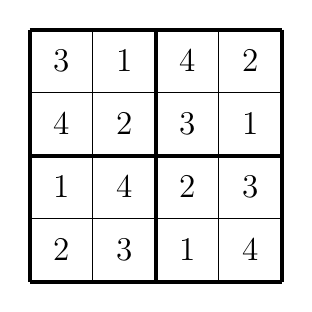
\begin{tikzpicture}[scale=0.8]
		\foreach \x in {0,2,4} \draw[line width=1.5pt] (\x,0)--(\x,-4);
		\foreach \x in {0,-2,-4} \draw[line width=1.5pt] (0,\x)--(4,\x);
		\foreach \x in {1,3} \draw (\x,0)--(\x,-4);
		\foreach \x in {-1,-3} \draw (0,\x)--(4,\x);
		\draw
		(1.5, -.5) node{\large $1$}
		(.5, -1.5) node{\large $4$}
		(1.5, -1.5) node{\large $2$}
		(1.5, -3.5) node{\large $3$}
		(2.5, -2.5) node{\large $2$}
		(.5, -.5) node{\large \bf $3$}
		(1.5, -2.5) node{\large \bf $4$}
		(.5, -2.5) node{\large \bf $1$}
		(.5, -3.5) node{\large \bf $2$}
		(3.5, -2.5) node{\large \bf $3$}
		(2.5, -1.5) node{\large $3$}
		(3.5, -1.5) node{\large \bf $1$}
		(2.5, -.5) node{\large \bf $4$}
		(3.5, -.5) node{\large \bf $2$}
		(2.5, -3.5) node{\large \bf $1$}
		(3.5, -3.5) node{\large \bf $4$}
		;
	\end{tikzpicture}
	\end{center}	
	
\end{Answer}
\begin{Answer}{9}
		$a)$	Các tập hợp con của $P$ có
		
		$\bullet$	1 phần tử là: $\{3\}$; $\{5\}$; $\{7\}$.
		
		$\bullet$	2 phần tử là: $\{3; 5\}$; $\{3; 7\}$; $\{5; 7\}$.
		
		$\bullet$	3 phần tử là: $\{3; 5; 7\}$.
		
		$b)$	Tập hợp rỗng cũng là tập con của tập hợp $P$. Do đó, tập hợp $P$ có tất cả 8
		tập hợp con.
	
\end{Answer}
\begin{Answer}{10}
		Từ trang 3 đến trang 9 dùng hết:
		\[(9 - 3) + 1 = 7 \text{(chữ số)}.\]
		Từ 10 đến 99 có: $(99 - 10) + 1 = 90$ (số). Do đó, số chữ số cần dùng là:
		\[90 \times 2 = 180 \text{(chữ số)}.\]
		Khi đó còn lại: $592 - 7 - 180 = 405 < 900$ (chữ số). Do đó số trang của cuốn sách là một số có 3 chữ số.
		
		Số trang sách kể từ 100 trở đi của cuốn sách đó là:
		\[405 : 3 = 135 \text{(trang)}.\]
		Khi đó, số trang của cuốn sách là
		\[100 + 135 - 1 = 234 \text{(trang)}.\]
		Vậy cuốn sách đó có 234 trang.
	
\end{Answer}
\begin{Answer}{11}
		Vì có 15 em thi đấu cờ vua trong 24 em của đội tuyển đấu cờ nên số em chỉ thi đấu cờ tướng là:
		\[24 - 15 = 9 \text{(em)}.\]
		Vì có 11 em thi đấu cờ tướng trong 24 em của đội tuyển đấu cờ nên số em chỉ thi đấu cờ vua là:
		\[24 - 11 = 13 \text{(em)}.\]
		Do đó, số em trong đội tuyển thi đấu cả hai môn là:
		\[11 - 9 = 2 = 15 - 13 \text{(em)}.\]
		Vậy có 2 em trong đội tuyển thi đấu cả hai môn.
	
\end{Answer}
\begin{Answer}{12}
		Gọi $A$ là tập hợp các đại biểu nói được tiếng Anh, $Đ$ là tập hợp các đại biểu nói được tiếng Đức, $P$ là tập hợp các đại biểu nói được tiếng Pháp. Ta có sơ đồ:
		\begin{center}
			\begin{tikzpicture}[scale=0.8]
				\draw
				(0:0) ellipse ({2.5} and {1.5})
				;
				\draw
				(-1,-2) circle (2cm);
				\draw
				(4:-2) ellipse ({2.5} and {1.5})
				;
				\draw
				(-4,1.5) node[left]{A}--(-3,1)
				(2.5,1.5) node[right]{Đ}--(1.5,1)
				(1.2,-3) node[right]{P}--(0,-2.5)
				;
				%	\foreach \i/\g in {a/0,b/0,1/0,2/60, c/-30}\fill[black] (\i) circle (2pt) +(\g:.4) node{$\i$};
			\end{tikzpicture}
		\end{center}
		Vì $39$ đại biểu nói được tiếng Pháp nên số đại biểu không nói được tiếng Pháp là
		\[100 - 39 = 61 \text{(đại biểu)}.\]
		Các đại biểu không nói được tiếng Pháp bao gồm: các đại biểu chỉ nói được tiếng Anh, các đại biểu chỉ nói được tiếng Đức, các đại biểu nói được cả hai tiếng Anh và Đức (không nói được tiếng Pháp).
		
		Vì 35 đại biểu chỉ nói được tiếng Anh và 8 đại biểu nói được cả hai tiếng Anh và Đức (không nói được tiếng Pháp) nên số đại biểu chỉ nói được tiếng Đức là:
		\[61 - 35 - 8 = 18 \text{(đại biểu)}.\]
		Vậy có 18 đại biểu chỉ nói được tiếng Đức.	
	
\end{Answer}
\begin{Answer}{13}
		\,\\
		\begin{center}
			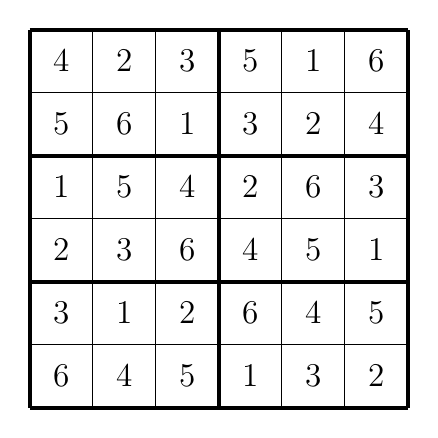
\begin{tikzpicture}[scale=0.8]
			\foreach \x in {0,3,6} \draw[line width=1.5pt] (\x,0)--(\x,6);
			\foreach \x in {0,2,4,6} \draw[line width=1.5pt] (0,\x)--(6,\x);
			\foreach \x in {1,2,4,5} \draw (\x,0)--(\x,6);
			\foreach \x in {1,3,5} \draw (0,\x)--(6,\x);
			\draw
			(1.5, .5) node{\large $4$}
			(3.5, .5) node{\large $1$}
			%
			(1.5, 1.5) node{\large $1$}
			(2.5, 1.5) node{\large $2$}
			(4.5, 1.5) node{\large $4$}
			(5.5, 1.5) node{\large \bf $5$}
			%
			(0.5, 2.5) node{\large \bf $2$}
			(2.5, 2.5) node{\large \bf $6$}
			(3.5, 2.5) node{\large \bf $4$}
			(4.5, 2.5) node{\large \bf $5$}
			%
			(1.5, 3.5) node{\large $5$}
			(2.5, 3.5) node{\large \bf $4$}
			(3.5, 3.5) node{\large \bf $2$}
			(5.5, 3.5) node{\large \bf $3$}
			%
			(.5, 4.5) node{\large \bf $5$}
			(1.5, 4.5) node{\large \bf $6$}
			(3.5, 4.5) node{\large \bf $3$}
			(4.5, 4.5) node{\large \bf $2$}
			%
			(2.5, 5.5) node{\large \bf $3$}
			(4.5,5.5) node{\large \bf $1$}
			%-----
			(0.5, 0.5) node{\large $6$}
			(2.5, 0.5) node{\large $5$}
			(4.5, 0.5) node{\large $3$}
			(5.5, 0.5) node{\large $2$}
			%
			(0.5, 1.5) node{\large $3$}
			(3.5, 1.5) node{\large $6$}
			%
			(1.5, 2.5) node{\large $3$}
			(5.5, 2.5) node{\large $1$}
			%
			(0.5, 3.5) node{\large $1$}
			(4.5, 3.5) node{\large $6$}
			%
			(2.5, 4.5) node{\large $1$}
			(5.5, 4.5) node{\large $4$}
			%
			(0.5, 5.5) node{\large $4$}
			(1.5, 5.5) node{\large $2$}
			(3.5, 5.5) node{\large $5$}
			(5.5, 5.5) node{\large $6$}
			;
		\end{tikzpicture}
		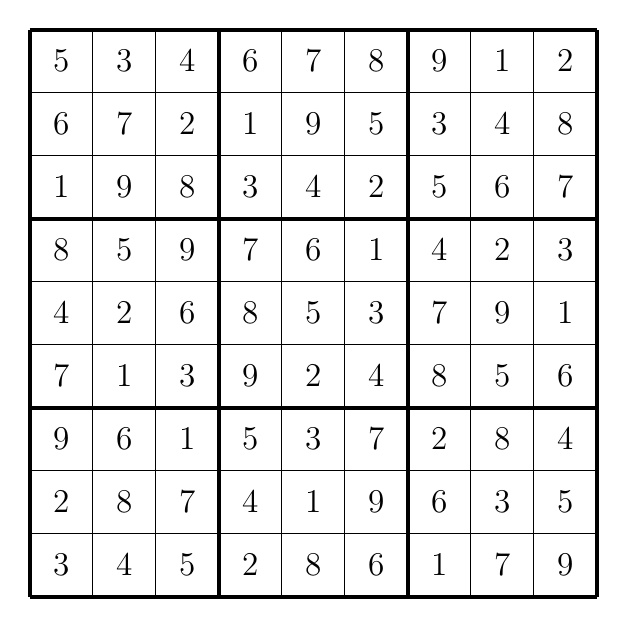
\begin{tikzpicture}[scale=.8]
			\foreach \x in {0,3,6,9} \draw[line width=1.5pt] (\x,0)--(\x,9);
			\foreach \x in {0,3,6,9} \draw[line width=1.5pt] (0,\x)--(9,\x);
			\foreach \x in {1,2,4,5,7,8} \draw (\x,0)--(\x,9);
			\foreach \x in {1,2,4,5,7,8} \draw (0,\x)--(9,\x);
			\draw
			(4.5, .5) node{\large $8$}
			(7.5, .5) node{\large $7$}
			(8.5, .5) node{\large $9$}
			%---
			(0.5, .5) node{\large $3$}
			(1.5, .5) node{\large $4$}
			(2.5, .5) node{\large $5$}
			(3.5, .5) node{\large $2$}
			(5.5, .5) node{\large $6$}
			(6.5, .5) node{\large $1$}
			%
			(3.5, 1.5) node{\large $4$}
			(4.5, 1.5) node{\large $1$}
			(5.5, 1.5) node{\large $9$}
			(8.5, 1.5) node{\large \bf $5$}
			%---
			(0.5, 1.5) node{\large $2$}
			(1.5, 1.5) node{\large $8$}
			(2.5, 1.5) node{\large $7$}
			(6.5, 1.5) node{\large \bf $6$}
			(7.5, 1.5) node{\large \bf $3$}
			%
			(1.5, 2.5) node{\large \bf $6$}
			(6.5, 2.5) node{\large \bf $2$}
			(7.5, 2.5) node{\large \bf $8$}
			%---
			(0.5, 2.5) node{\large \bf $9$}
			(2.5, 2.5) node{\large \bf $1$}
			(3.5, 2.5) node{\large \bf $5$}
			(4.5, 2.5) node{\large \bf $3$}
			(5.5, 2.5) node{\large \bf $7$}
			(8.5, 2.5) node{\large \bf $4$}
			%
			(0.5, 3.5) node{\large $7$}
			(4.5, 3.5) node{\large \bf $2$}
			(8.5, 3.5) node{\large \bf $6$}
			%---
			(1.5, 3.5) node{\large $1$}
			(2.5, 3.5) node{\large \bf $3$}
			(3.5, 3.5) node{\large \bf $9$}
			(5.5, 3.5) node{\large $4$}
			(6.5, 3.5) node{\large \bf $8$}
			(7.5, 3.5) node{\large \bf $5$}
			%
			(0.5, 4.5) node{\large \bf $4$}
			(3.5, 4.5) node{\large \bf $8$}
			(5.5, 4.5) node{\large \bf $3$}
			(8.5, 4.5) node{\large \bf $1$}
			%---
			(1.5, 4.5) node{\large \bf $2$}
			(2.5, 4.5) node{\large \bf $6$}
			(4.5, 4.5) node{\large \bf $5$}
			(6.5, 4.5) node{\large \bf $7$}
			(7.5, 4.5) node{\large \bf $9$}
			%
			(0.5, 5.5) node{\large \bf $8$}
			(4.5,5.5) node{\large \bf $6$}
			(8.5,5.5) node{\large \bf $3$}
			%---
			(1.5, 5.5) node{\large \bf $5$}
			(2.5,5.5) node{\large \bf $9$}
			(3.5,5.5) node{\large \bf $7$}
			(5.5, 5.5) node{\large \bf $1$}
			(6.5,5.5) node{\large \bf $4$}
			(7.5,5.5) node{\large \bf $2$}
			%
			(1.5,6.5) node{\large \bf $9$}
			(2.5,6.5) node{\large \bf $8$}
			(7.5,6.5) node{\large \bf $6$}
			%---
			(0.5,6.5) node{\large \bf $1$}
			(3.5,6.5) node{\large \bf $3$}
			(4.5,6.5) node{\large \bf $4$}
			(5.5,6.5) node{\large \bf $2$}
			(6.5,6.5) node{\large \bf $5$}
			(8.5,6.5) node{\large \bf $7$}
			%
			(0.5,7.5) node{\large \bf $6$}
			(3.5,7.5) node{\large \bf $1$}
			(4.5,7.5) node{\large \bf $9$}
			(5.5,7.5) node{\large \bf $5$}
			%---
			(1.5,7.5) node{\large \bf $7$}
			(2.5,7.5) node{\large \bf $2$}
			(6.5,7.5) node{\large \bf $3$}
			(7.5,7.5) node{\large \bf $4$}
			(8.5,7.5) node{\large \bf $8$}
			%
			(0.5,8.5) node{\large \bf $5$}
			(1.5,8.5) node{\large \bf $3$}
			(4.5,8.5) node{\large \bf $7$}
			%---
			(2.5,8.5) node{\large \bf $4$}
			(3.5,8.5) node{\large \bf $6$}
			(5.5,8.5) node{\large \bf $8$}
			(6.5,8.5) node{\large \bf $9$}
			(7.5,8.5) node{\large \bf $1$}
			(8.5,8.5) node{\large \bf $2$}
			;
		\end{tikzpicture}
		\end{center}
	
\end{Answer}
\begin{Answer}{14}
		Vì $abc$ là số lẻ nên $c \in \{1; 3; 5; 7; 9\}$.
		
		Do $a < b \le c$ và $a + b + c = 21$ nên ta xét $c = 9$ trước. Khi đó, ta có các trường hợp:
		
		$\bullet$	$b = c = 9 \Rightarrow a = 3$. Ta được số 399.
		
		$\bullet$	$c = 9; b = 8 \Rightarrow a = 4$. Ta được số 489.
		
		$\bullet$	$c = 9; b = 7 \Rightarrow a = 5$. Ta được số 579.
		
		Xét $c = 7 \Rightarrow a = b = c = 7$ không thỏa mãn đề bài.
		
		Vậy có 3 số tự nhiên lẻ có ba chữ số thỏa mãn đề bài.
	
\end{Answer}
